\chapter{图灵机}

\section{图灵机}

\subsection{艾伦·麦席森·图灵(Alan Mathison Turing)}

在1900年的巴黎国际数学大会上,数学家希尔伯特(David Hilbert)提出23个重要的数学问题,其中第十个是“随便给一个不确定的方程,能够通过有限步的运算,判断它是否存在整数解?”\\

如果这个问题的答案是否定的,那么意味着有些问题是无解的。正是因为对这个问题的深刻认识,让图灵认识到计算机的能力存在极限。\\

后来在1970年,前苏联伟大的数学家马季亚谢维奇从数学上解决了希尔伯特的那个问题。也就是说,的确有很多数学问题,根本没有答案,而且这样的问题比有答案的问题还要多得多。\\

\begin{figure}[H]
    \centering
    \begin{tikzpicture}
        \draw[fill=gray] (0,0) circle (4);
        \draw[fill=yellow] (0,-1) circle (3);
        \draw[fill=blue] (0,-2) circle (2);
        \draw[fill=purple] (0,-3) circle (1);
        \draw[fill=orange] (0,-3.5) circle (0.5);
        \draw[fill=green] (0,-3.75) circle (0.25);

        \node at (6.5,2) {\textcolor{gray}{所有问题}:};
        \node at (6.5,1) {\textcolor{yellow}{数学问题}};
        \node at (6.5,0) {\textcolor{blue}{可计算问题}};
        \node at (6.5,-1) {\textcolor{purple}{图灵机能解决的问题}};
        \node at (6.5,-2) {\textcolor{orange}{AI能解决的问题}};
        \node at (6.5,-3) {\textcolor{green}{AI已经找到解决方法的问题}};
    \end{tikzpicture}
    \caption{数学问题的分类}
\end{figure}

\vspace{0.5cm}

\subsection{图灵机(Turing Machine)}

1935年,22岁的图灵写出了\textit{On computable numbers, with an application to the Entscheidungsproblem},并从数学和逻辑上定义了著名的图灵机。今天所有的计算机,包括全世界正在设计的新的计算机,从解决问题的能力来讲,都没有超出图灵机的范畴。\\

图灵机是图灵构想出来的虚拟机器,这个机器的伟大之处在于,它非常简单,但是却可以模拟任何的计算机程序。\\

\begin{figure}[H]
    \centering
    \includegraphics[scale=3]{img/C3/3-1/1.png}
    \caption{图灵机}
\end{figure}

任何能被数字计算机执行的事情,图灵机同样也能够完成。如果你能写出一个算法来解决某个问题,那么同样可以写出一个图灵机程序来解决相同的问题。\\

图灵机的结构包括:

\begin{itemize}
    \item 存储带(tape)
          \begin{itemize}
              \item 双向无限延长
              \item 存储带上有一个个小方格,每个小方格里面存储一个符号
          \end{itemize}

    \item 控制器
          \begin{itemize}
              \item 可以存储图灵机当前自身的状态
              \item 可以改变自身的状态
              \item 包含一个读写头(read-write head),可以读、写存储带上方格里面的内容
              \item 读写头可以沿着存储带一格一格地左移或者右移。
          \end{itemize}
\end{itemize}

这里存储带其实就相当于现在计算机的内存,控制器相当于CPU和程序代码。\\

\begin{figure}[H]
    \centering
    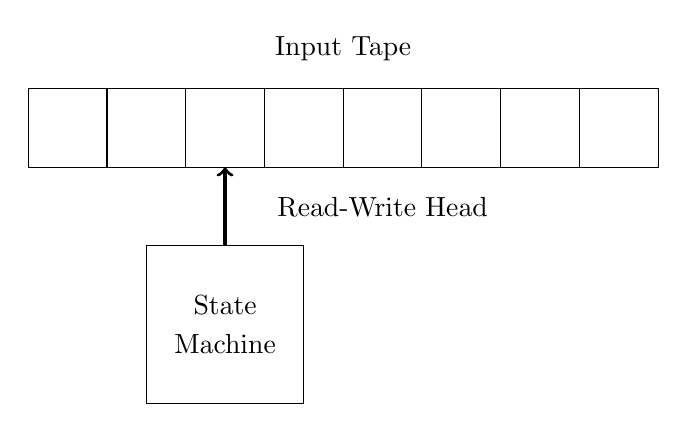
\begin{tikzpicture}
        \node at (4,1.5) {Input Tape};
        \draw (0,0) rectangle (8,1);
        \draw[-] (1,0) -- (1,1);
        \draw[-] (2,0) -- (2,1);
        \draw[-] (3,0) -- (3,1);
        \draw[-] (4,0) -- (4,1);
        \draw[-] (5,0) -- (5,1);
        \draw[-] (6,0) -- (6,1);
        \draw[-] (7,0) -- (7,1);

        \draw (1.5,-3) rectangle (3.5,-1);
        \node at (2.5,-1.75) {State};
        \node at (2.5,-2.25) {Machine};

        \draw[->, very thick] (2.5,-1) -- (2.5,0);
        \node at (4.5,-0.5) {Read-Write Head};
    \end{tikzpicture}
    \caption{图灵机}
\end{figure}

在运行图灵机前,首先需要将输入放入存储带中,然后将图灵机的状态设置为初始状态。开始运行后,图灵机会对存储带上的字符进行读写,当图灵机停止后,结果将会留在存储带上。\\

$ \delta $是图灵机的状态转换函数。\\

例如将当前字符$ a $替换为$ b $,并左移一格,可表示为$ \delta(q_i, a) = (q_j, b, L) $。

\begin{figure}[H]
    \centering
    \begin{tikzpicture}
        \node[state] (qi) {$ q_i $};
        \node[state] (qj) at (5,0) {$ q_j $};
        \draw (qi) edge[above] node{$ a/b, L $} (qj);
    \end{tikzpicture}
\end{figure}

例如将当前字符$ a $替换为$ b $,并右移一格,可表示为$ \delta(q_i, a) = (q_j, b, R) $。

\begin{figure}[H]
    \centering
    \begin{tikzpicture}
        \node[state] (qi) {$ q_i $};
        \node[state] (qj) at (5,0) {$ q_j $};
        \draw (qi) edge[above] node{$ a/b, R $} (qj);
    \end{tikzpicture}
\end{figure}

如果$ a = b $,则用$ a, L $或$ a, R $表示。\\

例如使用图灵机进行加法运算,为了方便操控图灵机,可将运算数转换为一进制的形式,如$ 2 + 3 $表示为$ 11 + 111 $。\\

在输入带上放入这两个运算数,中间用$ 0 $作为分割。输入内容的两端放入$ \Diamond $,用于标记开始和结束位置。\\

\begin{figure}[H]
    \centering
    \begin{tikzpicture}
        \draw (0,0) rectangle (10,1);
        \draw[-] (1,0) -- (1,1);
        \draw[-] (2,0) -- (2,1);
        \draw[-] (3,0) -- (3,1);
        \draw[-] (4,0) -- (4,1);
        \draw[-] (5,0) -- (5,1);
        \draw[-] (6,0) -- (6,1);
        \draw[-] (7,0) -- (7,1);
        \draw[-] (8,0) -- (8,1);
        \draw[-] (9,0) -- (9,1);

        \draw[->, very thick] (2.5,-1) -- (2.5,0);
        \node at (2.5,-1.5) {$ q_0 $};

        \node at (1.5,0.5) {$ \Diamond $};
        \node at (2.5,0.5) {$ 1 $};
        \node at (3.5,0.5) {$ 1 $};
        \node at (4.5,0.5) {$ 0 $};
        \node at (5.5,0.5) {$ 1 $};
        \node at (6.5,0.5) {$ 1 $};
        \node at (7.5,0.5) {$ 1 $};
        \node at (8.5,0.5) {$ \Diamond $};
    \end{tikzpicture}
\end{figure}

用于计算加法的图灵机可表示为:

\begin{figure}[H]
    \centering
    \begin{tikzpicture}
        \node[state, initial] (q0) {$ q_0 $};
        \node[state] (q1) at (3.5,0) {$ q_1 $};
        \node[state] (q2) at (7,0) {$ q_2 $};
        \node[state] (q3) at (10.5,0) {$ q_3 $};
        \node[state, accepting] (q4) at (8,-2) {$ q_4 $};

        \draw (q0) edge[loop above] node{$ 1 \rightarrow 1, R $} (q0)
        (q0) edge[above] node{$ 0 \rightarrow 1, R $} (q1)
        (q1) edge[loop above] node{$ 1 \rightarrow 1, R $} (q1)
        (q1) edge[above] node{$ \Diamond \rightarrow \Diamond, L $} (q2)
        (q2) edge[above] node{$ 1 \rightarrow 0, L $} (q3)
        (q3) edge[loop above] node{$ 1 \rightarrow 1, L $} (q3)
        (q3) edge[right] node{$ \Diamond \rightarrow \Diamond, R $} (q4);
    \end{tikzpicture}
\end{figure}

当图灵机停止后,输入带中的内容即为最终结果。\\

\begin{figure}[H]
    \centering
    \begin{tikzpicture}
        \draw (0,0) rectangle (10,1);
        \draw[-] (1,0) -- (1,1);
        \draw[-] (2,0) -- (2,1);
        \draw[-] (3,0) -- (3,1);
        \draw[-] (4,0) -- (4,1);
        \draw[-] (5,0) -- (5,1);
        \draw[-] (6,0) -- (6,1);
        \draw[-] (7,0) -- (7,1);
        \draw[-] (8,0) -- (8,1);
        \draw[-] (9,0) -- (9,1);

        \draw[->, very thick] (2.5,-1) -- (2.5,0);
        \node at (2.5,-1.5) {$ q_4 $};

        \node at (1.5,0.5) {$ \Diamond $};
        \node at (2.5,0.5) {$ 1 $};
        \node at (3.5,0.5) {$ 1 $};
        \node at (4.5,0.5) {$ 1 $};
        \node at (5.5,0.5) {$ 1 $};
        \node at (6.5,0.5) {$ 1 $};
        \node at (7.5,0.5) {$ 0 $};
        \node at (8.5,0.5) {$ \Diamond $};
    \end{tikzpicture}
\end{figure}

借助图灵机模拟器\url{http://turingmachine.vassar.edu/EZzvuYfv8}可以可视化运行过程。

\newpage

\section{停机问题}

\subsection{不可判定性(Undecidability)}

世界上存在不可解问题,存在数学和程序都不能抵达的边界。\\

图灵当年想要证明希尔伯特的可判定性问题,也就是说,是否存在一种通用的机械过程,能够判定任何数学命题的真假。\\

于是图灵就设计了一种假象的机器,也就是图灵机。他首先证明,图灵机就覆盖了所有的机械过程。如果存在一个问题,图灵机判定不了,那么就说明,不存在这种通用的机械过程,这样就证明了原问题。\\

然后,图灵就设计了一个问题,确实是图灵机判定不了的,这个问题就是“对于一个输入,让图灵机判定自己是否能够在有限的时间内停下来”。\\

经过证明,这个问题是图灵机回答不了的,所以原问题得以证否。这个问题被称为停机问题(Halting Problem)。\\

图灵当时设计这个图灵机,完全只是为了辅助他证明这个问题而已,这个机器是假想的、不存在的。可是后来他又发现,虽然这个机器不能解决所有的问题,但确实能够解决很多问题,而且真的是可以造出来的。\\

\subsection{理发师悖论}

停机问题类似于理发师悖论。\\

在一座小岛上有位理发师,有一天他做出一项规定:“他只给岛上所有不自己理发的人理发”。随着这个理发师自己的头发越来越长,他发现自己陷入了一个两难的境地:他该不该给自己理发?\\

如果他不为自己理发,按照他的规则,他属于自己的服务客户范围,因此可以给自己理发;如果他选择为自己理发,同样按照规则,他便不属于自己的服务对象,因此他又不能给自己理发。\\

\subsection{停机问题}

在写代码时,有时会遇到一个程序一直在运行,等了半天毫无反应。但是我们不知道程序是陷入了死循环导致根本不会停止,还是仅仅只是运行时间很久。\\

如果一个程序能够有限时间内运行完,就认为是可停机的。这个有限时间是个理论的概念,无论是1秒还是200亿年,只要有终止的时候,就是可停机的。\\

因此,如果存在一种程序,能够判断一个程序是否可停机,那么就可以解决上面的问题。遗憾的是,不存在这样的一个程序使得其能判断任意程序的停机问题,即停机问题不可判定。\\

可以利用反证法进行证明。假设存在这样一个程序$ H $,能够判断任何一个程序是否可以停机,即$ H $的判断总是正确的。\\

那么,我们可以设计一个程序$ X $,它的功能是让$ H $判断$ X $本身能否停机,并将结果取反(即如果可以停机则输出不可停机;如果不可停机则输出可停机)。\\

这样就得到了一个悖论:

\begin{enumerate}
    \item 如果$ H $得出的结果是可停机的,但是$ X $输出的结果是不可停机,说明$ H $判断错了。
    \item 如果$ H $得出的结果是不可停机的,但是$ X $输出的结果是可停机,说明$ H $判断错了。
\end{enumerate}

因此,并不存在$ H $这样一个程序,能够判断任意程序的停机问题。\\

通过动画\url{https://www.youtube.com/watch?v=92WHN-pAFCs}可以更直观地理解停机问题。

\newpage